\documentclass[mathserif,11pt]{beamer}

\usepackage{url,verbatim,natbib}
\usepackage[english]{babel}
\usepackage{amsmath, mathabx}
\usepackage{dsfont, ulem}
\usepackage{tikz}
\usepackage{xparse}
\newtheorem{proposition}[theorem]{Proposition}

\usepackage[headheight=22pt]{beamerthemeboxes}
\usepackage{graphicx}
\beamertemplatenavigationsymbolsempty 
\setbeamercovered{transparent}
\usepackage{centernot}

\setbeamertemplate{itemize item}{$\bullet$} 
\setbeamercolor{title}{fg=uio}
\setbeamertemplate{sections/subsections in toc}[ball unnumbered]
\setbeamercolor{section in toc}{fg=uio,bg=white}
\setbeamercolor{subsection in toc}{fg=uio,bg=white}
\setbeamercolor{result}{fg=black, bg=yellow}
\newcommand{\dotsim}{\stackrel{\cdot}{\sim}}
\newcommand{\interi}{{\rm Z}\negthinspace\negthinspace {\rm Z}}
\newcommand{\reali}{{\rm I}\negthinspace {\rm R}}
\newcommand{\naturali}{{\rm I}\negthinspace {\rm N}}
\newcommand{\sign}{\mathop{\rm sgn}\nolimits}
\newcommand{\sgn}{\mathop{\mathrm{sgn}}}
\definecolor{redve}{rgb}{0.604,0.008,0.00}
\definecolor{lmu}{rgb}{0.188,0.522,0.306}
\definecolor{uio}{rgb}{0.847,0.118,0.02}

\def\R{{\rm I\!R}}
\def\P{{\rm Pr}}
\def\Real{{\rm I\!R}}
\def\T{{\footnotesize {^{_{\sf T}}}}}
\def\tr{{\rm tr}}
\def\diag{{\rm diag}}

\NewDocumentCommand\DownArrow{O{2.0ex} O{black}}{%
   \mathrel{\tikz[baseline] \draw [<-, line width=0.5pt, #2] (0,0) -- ++(0,#1);}
}

\useframetitletemplate{% 
\begin{centering} 
\begin{small} \structure{\textcolor{uio} \insertframetitle {\insertframesubtitle}}
\end{small}

\end{centering} 
}

\addheadboxtemplate{\color[rgb]{1,1,1}}{\color{uio} \underline{{\hspace{5pt}\includegraphics[scale=0.06]{../../../../support/uio_logo_eng} \hspace{0.265\paperwidth}\color{black} \tiny  STK-IN4300 - Statistical Learning Methods in Data Science} \hspace{5pt}}}

%\bfseries{\insertsection}

\addfootboxtemplate{\color[rgb]{1,1,1}}{\color{black} \tiny \quad  
STK-IN4300: lecture 7
  \hfill \tiny \insertframenumber / \inserttotalframenumber \hspace{5pt}}

  
\title{STK-IN4300 \\ Statistical Learning Methods in Data Science}
\author{Riccardo De Bin} 
\institute{debin@math.uio.no} 
\date{}


\begin{document}
\setbeamercolor{bgr}{fg=black,bg=uio}

{
\setbeamertemplate{headline}{}
\frame{
\vspace{-2cm}
\begin{beamercolorbox}[sep=-2.2em,wd=5cm,colsep=0.5pt,ht=4.25ex,dp=3ex,left]{postit}
\includegraphics[scale=0.06]{../../../../support/uio_logo_eng}
\end{beamercolorbox}
\vspace{0.365cm}
\noindent\makebox[\linewidth]{\color{uio} \rule{\paperwidth}{0.4pt}}
\vspace{2.5cm}
\titlepage
}
}

\frame{\frametitle{Outline of the lecture}
\tableofcontents
}


\section{Basis Expansions and Regularization}

\subsection{Piecewise polynomials and splines}

\frame{\frametitle{Piecewise polynomials and splines: }
\framesubtitle{beyond linear regression}
For regression problems:
\begin{itemize}
\item usually $f(X)=E[Y|X]$ is considered \textcolor{uio}{linear in $X$}:
\begin{itemize}
\item easy and convenient \textcolor{uio}{approximation};
\item \textcolor{uio}{first Taylor} expansion;
\item model easy to \textcolor{uio}{interpret};
\item \textcolor{uio}{smaller variance} (fewer parameter to be estimated);
\end{itemize}
\item often in reality $f(X)$ is \textcolor{uio}{not linear} in $X$;
\item IDEA: use \textcolor{uio}{transformations} of $X$ to capture \textcolor{uio}{non-linearity} and fit a linear model in the new derived input space.
\end{itemize}
}


\frame{\frametitle{Piecewise polynomials and splines: }
\framesubtitle{linear basis expansion}
Consider the following model (\textcolor{uio}{linear basis expansion} in $X$),
$$
f(X) = \sum_{m=1}^M \beta_m h_m(X),
$$
where $h_m(X):\mathds{R}^p \rightarrow \mathds{R}$s denote the $m$-th transformation of X.

\vspace{12pt}

Note:
\begin{itemize}
\item the new variables $h_m(X)$ \textcolor{uio}{replace} $X$ in the regression;
\item the new model is \textcolor{uio}{linear} in the new variables;
\item \textcolor{uio}{usual} fitting procedures are used.
\end{itemize}
}


\frame{\frametitle{Piecewise polynomials and splines: }
\framesubtitle{choices of $h_m(X)$}
Typical choices of $h_m(X)$:
\begin{itemize}
\item $h_m(X) = X_m$: \textcolor{uio}{original} linear model;
\item $h_m(X) = X_j^2$ or $h_m(X) = X_jX_k$: \textcolor{uio}{polynomial} terms,
\begin{itemize}
\item augmented space to achieve \textcolor{uio}{higher-order Taylor} expansions;
\item the number of variables \textcolor{uio}{grow exponentially} ($O(p^d)$, where $d$ is the order of the polynomial, $p$ the number of variables);
\end{itemize}
\item $h_m(X) = \log(X_j), \sqrt{X_j}, \dots$: \textcolor{uio}{non-linear} transformations;
\item $h_m(X) = \mathds{1}(L_m \leq X_k < U_m)$: \textcolor{uio}{indicator} for a region of $X_k$,
\begin{itemize}
\item \textcolor{uio}{breaks} the range of $X_k$ into $M_k$ \textcolor{uio}{non-overlapping regions};
\item \textcolor{uio}{piecewise constant} contribution of $X_k$.
\end{itemize}
\end{itemize}
}


\frame{\frametitle{Piecewise polynomials and splines: }
\framesubtitle{introduction}
Remarks:
\begin{itemize}
\item particular functional forms (e.g., logarithm) are useful in \textcolor{uio}{specific} situations;
\item polynomial forms are more \textcolor{uio}{flexible} but \textcolor{uio}{limited} by their global nature;
\item[]
\item \textcolor{uio}{piecewise-polynomials} and \textcolor{uio}{splines} allow for \textcolor{uio}{local} polynomials;
\item the class of functions is \textcolor{uio}{limited},
\begin{align*}
f(X) &= \sum_{j=1}^p f_j(X_j)\\
  &= \sum_{j=1}^p \sum_{m=1}^M \beta_{jm} h_{jm}(X_j),
\end{align*}
by the number of basis $M_j$ used for each component $f_j$.
\end{itemize}
}


\frame{\frametitle{Piecewise polynomials and splines: }
\framesubtitle{piecewise constant}
\begin{columns}
\begin{column}{0.5\textwidth}
The {\bf \uline{piecewise constant}} function:
\begin{itemize}
\item \textcolor{uio}{simplest} solution;
\item three basis functions:
\begin{itemize}
\item $h_1(X) = \mathds{1}(X < \xi_1)$
\item $h_2(X) = \mathds{1}(\xi_1 \leq X < \xi_2)$
\item $h_3(X) = \mathds{1}(\xi_2 \leq X)$
\end{itemize}
\item disjoint regions;
\item $f(X) = \sum_{m=1}^3 \beta_m h_m(X)$;
\item $\hat{\beta}_m = \bar{Y}_m$, the \textcolor{uio}{mean} of $Y$ in the region $m$.
\end{itemize}
\end{column}
\begin{column}{0.5\textwidth}
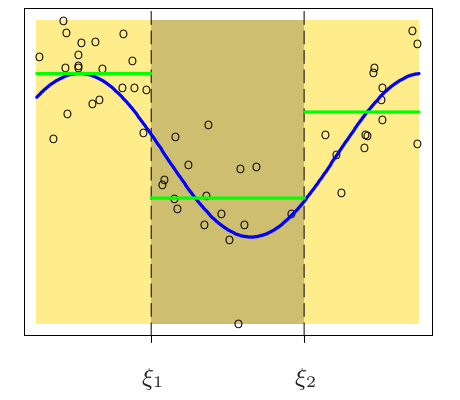
\includegraphics[width=1.1\textwidth]{figure5_1_tl}
\end{column}
\end{columns}
}


\frame{\frametitle{Piecewise polynomials and splines: }
\framesubtitle{piecewise linear}
\begin{columns}
\begin{column}{0.5\textwidth}
A {\bf \uline{piecewise linear}} fit:
\begin{itemize}
\item a \textcolor{uio}{linear fit} instead of a constant fit in each region;
\item three \textcolor{uio}{additional} basis functions:
\begin{itemize}
\item $h_4(X) = h_1(X)X$
\item $h_5(X) = h_2(X)X$
\item $h_6(X) = h_3(X)X$
\end{itemize}
\item $\hat{\beta}_1, \hat{\beta}_2, \hat{\beta}_3$ are the intercepts;
\item $\hat{\beta}_4, \hat{\beta}_5, \hat{\beta}_6$ are the slopes;
\end{itemize}
\end{column}
\begin{column}{0.5\textwidth}
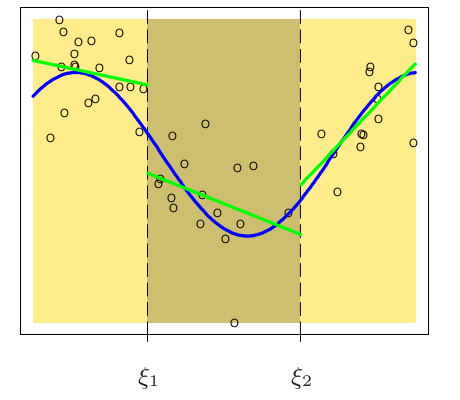
\includegraphics[width=1.1\textwidth]{figure5_1_tr}
\end{column}
\end{columns}
}


\frame{\frametitle{Piecewise polynomials and splines: }
\framesubtitle{piecewise linear}
\begin{columns}
\begin{column}{0.55\textwidth}
A {\bf \uline{continuous piecewise linear}} fit:
\begin{itemize}
\item \textcolor{uio}{force continuity} at knots;
\item generally \textcolor{uio}{preferred to the non-continuous} version;
\item add constrains,
\begin{itemize}
\item $\hat{\beta}_1 + \xi_1\hat{\beta}_4 = \hat{\beta}_2 + \xi_1\hat{\beta}_5$;
\item $\hat{\beta}_2 + \xi_2\hat{\beta}_5 = \hat{\beta}_3 + \xi_2\hat{\beta}_6$;
\end{itemize}
\item 2 restrictions $\rightarrow$ 4 free parameters;
\end{itemize}
\end{column}
\begin{column}{0.5\textwidth}
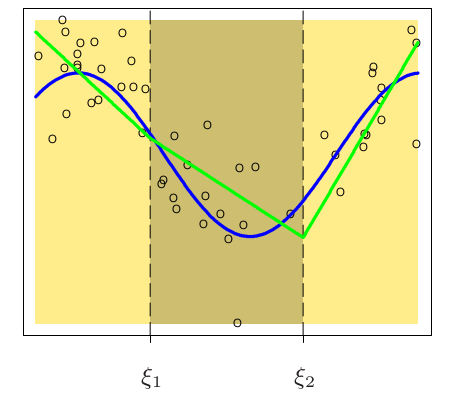
\includegraphics[width=1.1\textwidth]{figure5_1_bl}
\end{column}
\end{columns}
}


\frame{\frametitle{Piecewise polynomials and splines: }
\framesubtitle{piecewise linear}
\begin{columns}
\begin{column}{0.5\textwidth}
The constrain can be \textcolor{uio}{directly incorporated} into the basis functions,
\begin{itemize}
\item $h_1(X) = 1$
\item $h_2(X) = X$
\item $h_3(X) = (X - \xi_1)_+$
\item $h_4(X) = (X - \xi_2)_+$
\end{itemize}
where $(\cdot)_+$ denotes the \textcolor{uio}{positive part}.
\end{column}
\begin{column}{0.5\textwidth}
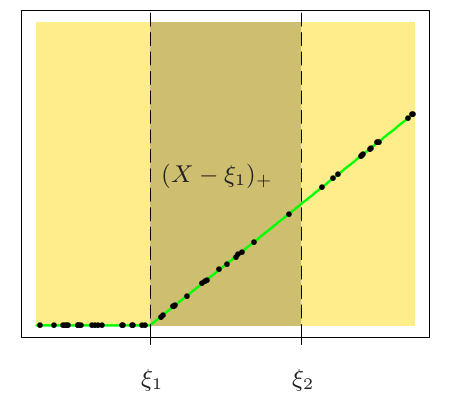
\includegraphics[width=1.1\textwidth]{figure5_1_br}
\end{column}
\end{columns}
}


\frame{\frametitle{Piecewise polynomials and splines: }
\framesubtitle{piecewise cubic polynomials}
\begin{columns}
\begin{column}{0.5\textwidth}
Further ``improvements'':
\begin{itemize}
\item \textcolor{uio}{smoother} functions;
\item increase the \textcolor{uio}{order} of the polynomials;
\item e.g., a \textcolor{uio}{cubic polynomial} in each disjoint region;
\item[] \centering $\downarrow$
\item[] \centering {\bf \uline{discontinuous piecewise cubic}} polynomials.
\end{itemize}
\end{column}
\begin{column}{0.5\textwidth}
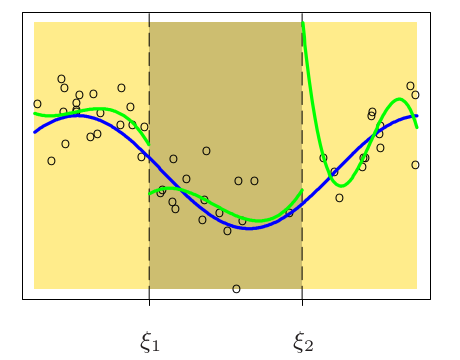
\includegraphics[width=1.1\textwidth]{figure5_2_tl}
\end{column}
\end{columns}
}


\frame{\frametitle{Piecewise polynomials and splines: }
\framesubtitle{piecewise cubic polynomials}
\begin{columns}
\begin{column}{0.5\textwidth}
Also in this case:
\begin{itemize}
\item we can \textcolor{uio}{force} the function to be \textcolor{uio}{continuous} at the nodes;
\item by \textcolor{uio}{adding constrains};
\item[] \centering $\downarrow$
\item[] \centering {\bf \uline{continuous piecewise cubic}} polynomials.
\end{itemize}
\end{column}
\begin{column}{0.5\textwidth}
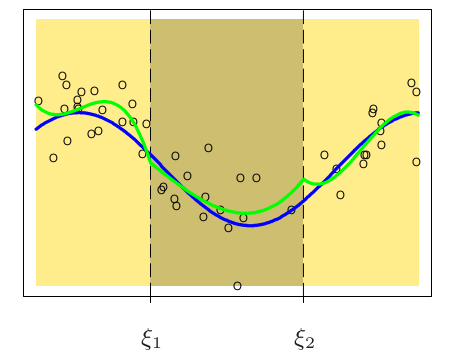
\includegraphics[width=1.1\textwidth]{figure5_2_tr}
\end{column}
\end{columns}
}


\frame{\frametitle{Piecewise polynomials and splines: }
\framesubtitle{piecewise cubic polynomials}
\begin{columns}
\begin{column}{0.52\textwidth}
Since we have third order polynomials:
\begin{itemize}
\item we can increase the \textcolor{uio}{order of continuity} at knots;
\item not only $f(\xi_k^-)=f(\xi_k^+)$;
\item \textcolor{uio}{additionally}, $f'(\xi_k^-)=f'(\xi_k^+)$.
\item[] \centering $\downarrow$
\item[] \centering {\bf \uline{first derivative continuous piecewise cubic}} polynomials.
\end{itemize}
\end{column}
\begin{column}{0.5\textwidth}
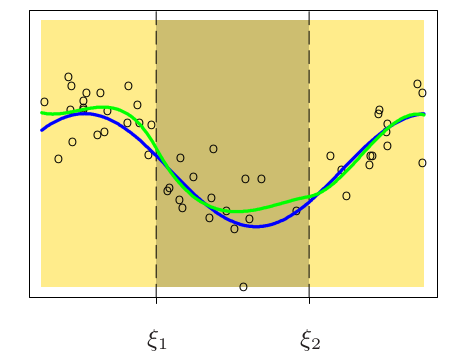
\includegraphics[width=1.1\textwidth]{figure5_2_bl}
\end{column}
\end{columns}
}


\frame{\frametitle{Piecewise polynomials and splines: }
\framesubtitle{piecewise cubic polynomials}
\begin{columns}
\begin{column}{0.5\textwidth}
Finally,
\begin{itemize}
\item \textcolor{uio}{further} increase the order of continuity;
\item constrain $f''(\xi_k^-)=f''(\xi_k^+)$
\item[] \centering $\downarrow$
\item[] \centering {\bf \uline{cubic splines}}.
\item[]
\item[]
\end{itemize}
\textcolor{uio}{Basis for cubic splines} with two knots $\xi_1$ and $\xi_2$:

\vspace{6pt}

\begin{tabular}{ccc}
$h_1(X) = 1$, & $h_3(X) = X^2$, & $h_5(X) = (X - \xi_1)^3_+$ \\
$h_2(X) = X$, & $h_4(X) = X^3$, & $h_6(X) = (X - \xi_2)^3_+$
\end{tabular}
\end{column}
\begin{column}{0.5\textwidth}
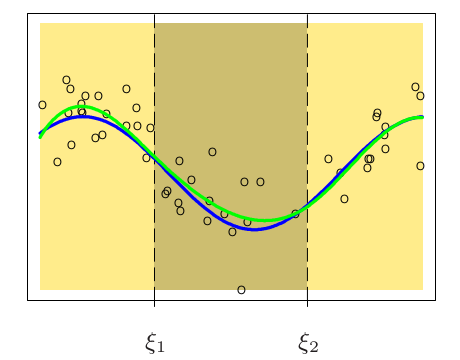
\includegraphics[width=1.1\textwidth]{figure5_2_br}
\end{column}
\end{columns}
}


\frame{\frametitle{Piecewise polynomials and splines: }
\framesubtitle{general order-M splines}
In general, an \textcolor{uio}{order-M spline} with knots $\xi_j$, $j=1,\dots,K$:
\begin{itemize}
\item is a \textcolor{uio}{piecewise-polynomial} of degree $M-1$;
\item has \textcolor{uio}{continuous derivatives} up to order $M-2$;
\item the \textcolor{uio}{general form} of the basis is:
\begin{align*}
h_j(X) &= X^{j-1}, j=1,\dots,M;\\
h_{M+\ell}(X) &= (X - \xi_\ell)^{M-1}_+, \ell=1,\dots,K;
\end{align*}
\item e.g., cubic spline $\rightarrow$ $M = 4$;
\item cubic splines are the \textcolor{uio}{lowest-order} spline for which the discontinuity at the knots \textcolor{uio}{cannot be seen} by a human eye
\item[] \centering $\Downarrow$
\item[] \centering no reason to use higher-order splines
\end{itemize}
}


\frame{\frametitle{Piecewise polynomials and splines: }
\framesubtitle{specifications}
For this kind of splines (a.k.a.\ regression splines), one needs:
\begin{itemize}
\item specify the \textcolor{uio}{order} of the \textcolor{uio}{spline};
\item select the \textcolor{uio}{number} of the \textcolor{uio}{knots};
\item choose their \textcolor{uio}{placement}.
\end{itemize}
Often:
\begin{itemize}
\item use cubic splines (\textcolor{uio}{$M = 4$});
\item use the \textcolor{uio}{degrees of freedom} to choose the number of knots;
\item e.g., for cubic splines,
\begin{itemize}
\item 4 degrees of freedom for the first cubic polynomial;
\item 1 degree of freedom for each knots ($4-1-1-1$);
\item \textcolor{uio}{number of basis = number of knots + 4};
\end{itemize}
\item use the \textcolor{uio}{$x_i$ to place} the knots;
\begin{itemize}
\item e.g., with 4 knots, $20^{th}, 40^{th}, 60^{th}, 80^{th}$ percentiles of $x$.
\end{itemize}
\end{itemize}
}


\frame{\frametitle{Piecewise polynomials and splines: }
\framesubtitle{natural cubic splines}
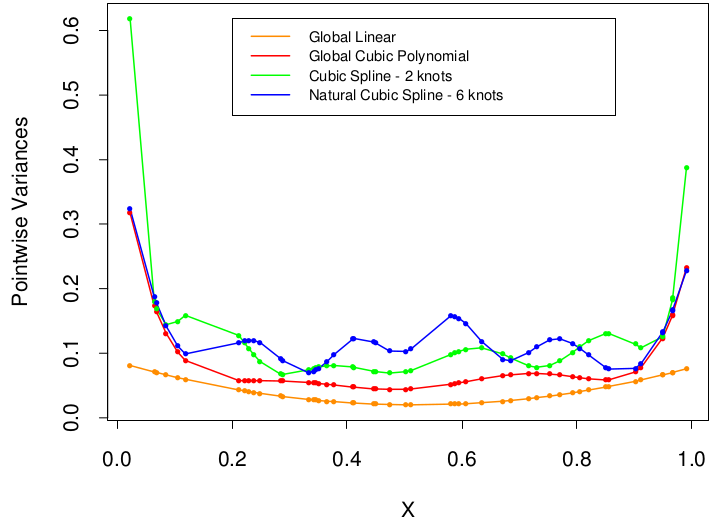
\includegraphics[width=0.95\textwidth]{figure5_3}
}


\frame{\frametitle{Piecewise polynomials and splines: }
\framesubtitle{natural cubic splines}
At the \textcolor{uio}{boundaries}:
\begin{itemize}
\item same \textcolor{uio}{issues} saw for kernel density;
\item \textcolor{uio}{high variance}.
\end{itemize}
Solution:
\begin{itemize}
\item force the function to be \textcolor{uio}{linear} beyond the \textcolor{uio}{boundary knots};
\item by adding \textcolor{uio}{additional constrains};
\item it \textcolor{uio}{frees up} 4 (2 for each boundary) degrees of freedom.
\end{itemize}
Basis (derived from those of the cubic splines):
$$
N_1(X) = 1 \quad\quad N_2(X) = X \quad\quad N_{k+2}(X) = d_k(X) - d_{K+1}
$$
where
$$
d_k = \frac{(X-\xi_k)^3_+ - (X-\xi_K)^3_+}{\xi_K-\xi_k}.
$$
}


\frame{\frametitle{Piecewise polynomials and splines: }
\framesubtitle{example}
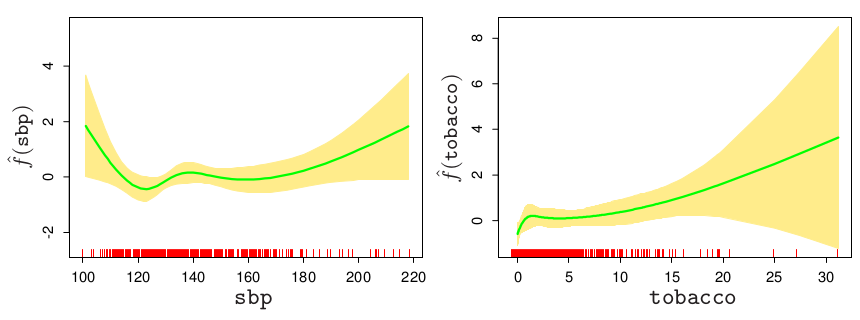
\includegraphics[width=\textwidth]{figure5_4_top}
}


\frame{\frametitle{Piecewise polynomials and splines: }
\framesubtitle{example}
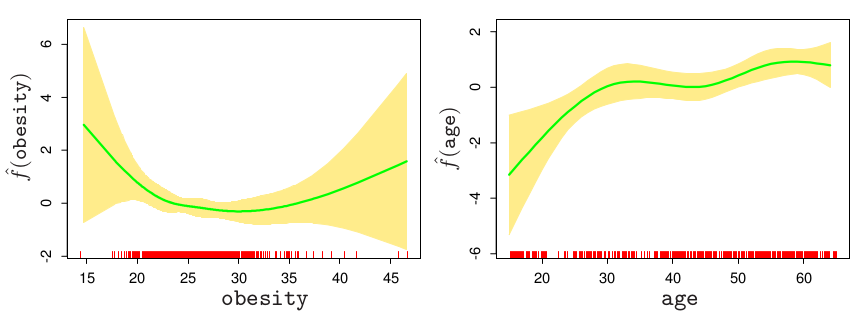
\includegraphics[width=\textwidth]{figure5_4_bottom}
}


\subsection{Smoothing splines}

\frame{\frametitle{Smoothing splines: }
\framesubtitle{introduction}
To \textcolor{uio}{avoid} choosing the number of knots and their placement:
\begin{itemize}
\item use the \textcolor{uio}{maximal number} (one for each observation);
\item control the complexity with a \textcolor{uio}{penalty term}.
\end{itemize}
}


\frame{\frametitle{Smoothing splines: }
\framesubtitle{minimizer}
Consider the \textcolor{uio}{minimization problem},
$$
\hat{f}(x) = \text{argmin}_{f(x)} \left\{\sum_{i=1}^N (y_i - f(x_i))^2 + \lambda\int\{f''(t)\}^2 dt \right\}
$$
such that $f(x)$ has \textcolor{uio}{two continuous derivatives}.

Here $\lambda$ is the \textcolor{uio}{smoothing parameter}:
\begin{itemize}
\item \textcolor{uio}{$\lambda=0$} $\rightarrow$ \textcolor{uio}{no constrain} ($f(x)$ can be any function \textcolor{uio}{interpolating} the data);
\item \textcolor{uio}{$\lambda=\infty$} $\rightarrow$ least squares line fit (\textcolor{uio}{no} curvature tolerated).
\end{itemize}

\vspace{12pt}

It can be shown that the \textcolor{uio}{unique minimizer} is a \textcolor{uio}{natural cubic spline} with knots at the unique values $x_i$, $i = 1, \dots, N$.
}


\frame{\frametitle{Smoothing splines: }
\framesubtitle{solution}
If we consider the \textcolor{uio}{natural spline}
$$
f(x) = \sum_{j=1}^N N_j(x)\theta_j,
$$
then
$$
\hat{\theta} = \text{argmin}_\theta \left\{(y-N\theta)^T(y-N\theta) + \lambda\theta^T\Omega_N\theta\right\},
$$
where:
\begin{itemize}
\item $\{N\}_{ij} = N_j(x_i)$, and $N_j(\cdot)$ are the basis functions;
\item $\{\Omega\}_{jk} = \int N_j''(t)N_k''(t)\;dt$.
\end{itemize}
Therefore,
$$
\hat{\theta} = (N^TN + \lambda\Omega_N)^{-1}N^Ty
$$
and
$$
\hat{f}(x) = \sum_{j=1}^N N_j(x)\hat{\theta}_j.
$$
}


\frame{\frametitle{Smoothing splines: }
\framesubtitle{example}
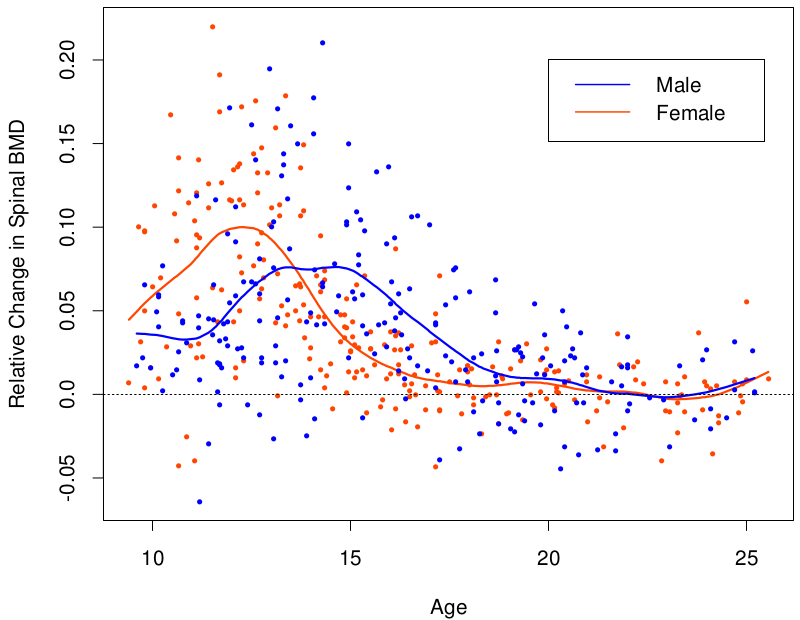
\includegraphics[width=0.9\textwidth]{figure5_6}
}


\subsection{Selection of the smoothing parameters}

\frame{\frametitle{Selection of the smoothing parameters: }
\framesubtitle{linear operators}
Polynomial splines and smoothing splines are \textcolor{uio}{linear operators}:
\begin{itemize}
\item cubic splines: $\hat{f}(x) = \underbrace{B_\xi(B^T_\xi B_\xi)^{-1}B^T_\xi}_{\textcolor{uio}{H_\xi}}y$;
\item smoothing splines: $\hat{f}(x) = \underbrace{N(N^TN+\lambda\Omega_N)^{-1}N^T}_{\textcolor{uio}{S_\lambda}}y$.
\end{itemize}
$H_\xi$ is called \textcolor{uio}{hat matrix}, $S_\lambda$ \textcolor{uio}{smoothing matrix}:
\begin{itemize}
\item they do \textcolor{uio}{not depend} on $y$ (linear [operator / smoother]);
\item are \textcolor{uio}{symmetric} and \textcolor{uio}{semidefinite positive};
\item $H_\xi H_\xi=H_\xi$ (\textcolor{uio}{idempotent}), $S_\lambda S_\lambda \preceq S_\lambda$ (\textcolor{uio}{shrinking});
\item \textcolor{uio}{$H_\xi$} has rank \textcolor{uio}{$M$}, \textcolor{uio}{$S_\lambda$} has rank \textcolor{uio}{$N$}.
\end{itemize}
}


\frame{\frametitle{Selection of the smoothing parameters: }
\framesubtitle{degrees of freedom}
The expression $M = \text{trace}(H_\xi)$ gives:
\begin{itemize}
\item the \textcolor{uio}{dimension} of the projection space;
\item \textcolor{uio}{number} of basis function;
\item \textcolor{uio}{number} of parameters involved in the fit.
\item[]
\end{itemize}
Similarly, we define the {\bf effective degrees of freedom} as
$$
\text{df}_\lambda = \text{trace}(S_\lambda).
$$
We can \textcolor{uio}{fix} the degrees of freedom and \textcolor{uio}{find} the value of $\lambda$:
\begin{itemize}
\item e.g., in the last example, $\text{df}_\lambda=12 \rightarrow \lambda = 2.2\times 10^{-4}$.
\end{itemize}
}


\frame{\frametitle{Selection of the smoothing parameters: }
\framesubtitle{example}
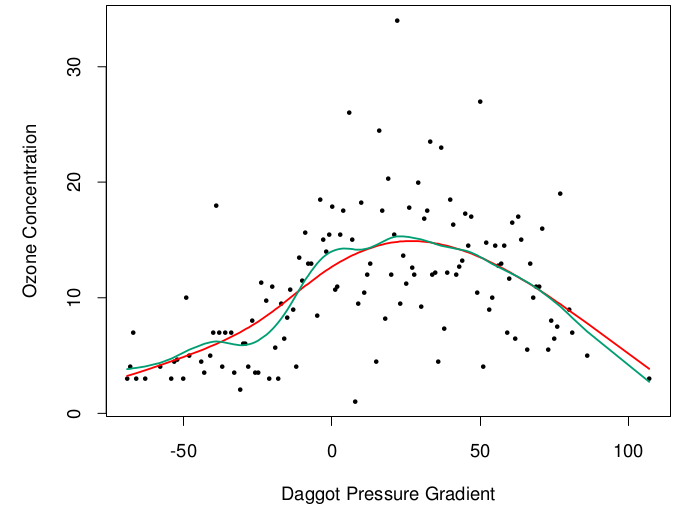
\includegraphics[width=0.98\textwidth]{figure5_7_top}
}


\frame{\frametitle{Selection of the smoothing parameters: }
\framesubtitle{example}
\centering
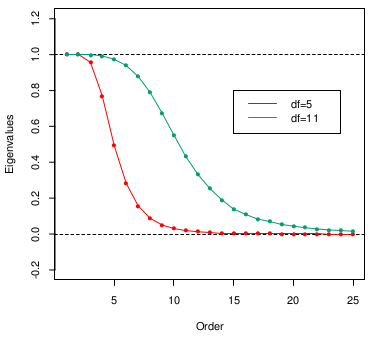
\includegraphics[width=0.75\textwidth]{figure5_7_bottom}
}


\frame{\frametitle{Selection of the smoothing parameters: }
\framesubtitle{example}
\centering
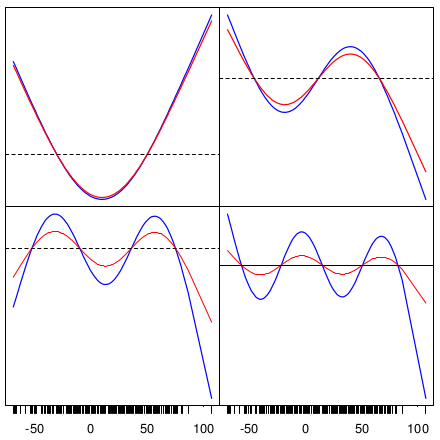
\includegraphics[width=0.7\textwidth]{figure5_7_br}
}


\frame{\frametitle{Selection of the smoothing parameters: }
\framesubtitle{smoother matrices}
Let us rewrite $S_\lambda$ in his \textcolor{uio}{Reinsch form},
$$
S_\lambda = (I + \lambda K)^{-1},
$$
where $K$ (\textcolor{uio}{penalty matrix}) does not depend on $\lambda$.

\vspace{12pt}

The \textcolor{uio}{eigen-decomposition} of $S_\lambda$ is
$$
S_\lambda = \sum_{k=1}^N \rho_k(\lambda)u_ku_k^T
$$
with $\rho_k(\lambda)=\frac{1}{1 + \lambda_k}$.
}


\frame{\frametitle{Selection of the smoothing parameters: }
\framesubtitle{smoother matrices}
Note that:
\begin{itemize}
\item the eigenvectors are \textcolor{uio}{not affected} by changes in $\lambda$,
\begin{itemize}
\item the \textcolor{uio}{whole family} of smoothing splines indexed by $\lambda$ has the \textcolor{uio}{same} eigenvectors;
\end{itemize}
\item $S_\lambda y = \sum_{k=1}^N u_k\rho_k(\lambda)\langle u_k,y \rangle$,
\begin{itemize}
\item smoothing splines \textcolor{uio}{decompose} $y$ w.r.t. the basis ${u_k}$;
\item differentially \textcolor{uio}{shrink} the contribution using $\rho_k(\lambda)$;
\end{itemize}
\item the eigenvalues $\rho_k(\lambda)=1/(1 + \lambda_k)$ are \textcolor{uio}{inverse function} of the eigenvalues $d_k$ of the penalty matrix $K$, \textcolor{uio}{moderated by $\lambda$},
\begin{itemize}
\item $\lambda$ \textcolor{uio}{controls the rate} at which $\rho_k(\lambda)$ decreases to 0.
\end{itemize}
\end{itemize}
}



\frame{\frametitle{Selection of the smoothing parameters: }
\framesubtitle{bias variance trade-off}
Consider the following example:
\begin{itemize}
\item $Y = f(X) + \epsilon$;
\item $f(X) = \frac{\sin(12(X+0.2))}{X+0.2}$;
\item $\epsilon \sim N(0,1)$;
\item $X \sim \text{Unif}[0,1]$;
\item $N=100$.
\item[]
\end{itemize}
We fit smoothing splines with \textcolor{uio}{three different values} of df$_\lambda$:
\begin{itemize}
\item $\text{df}_\lambda = 5$;
\item $\text{df}_\lambda = 9$;
\item $\text{df}_\lambda = 15$.
\end{itemize}
}


\frame{\frametitle{Selection of the smoothing parameters: }
\framesubtitle{bias variance trade-off}
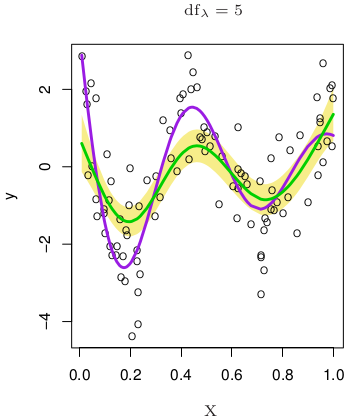
\includegraphics[width=0.33\textwidth]{figure5_9_tr}
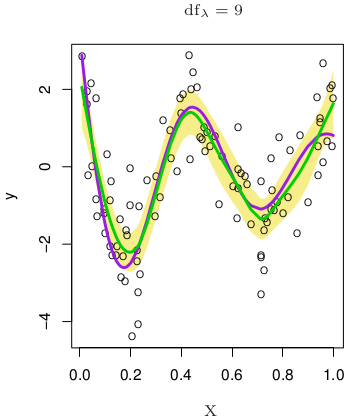
\includegraphics[width=0.33\textwidth]{figure5_9_bl}
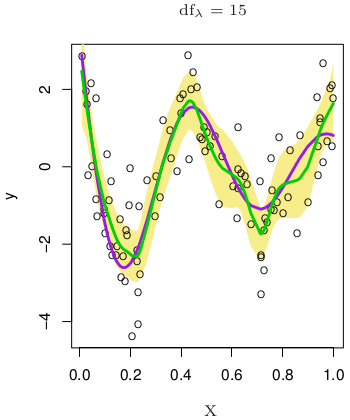
\includegraphics[width=0.33\textwidth]{figure5_9_br}
}


\frame{\frametitle{Selection of the smoothing parameters: }
\framesubtitle{bias variance trade-off}
In yellow it is shown the area \textcolor{uio}{$\hat{f}_\lambda(x) \pm 2\cdot se(\hat{f}_\lambda(x))$}.

\vspace{12pt}

Since $\hat{f}(x)=S_\lambda(x)y$,
$$
\text{Cov}(\hat{f}(x)) = S_\lambda \text{Cov}(y) S_\lambda^T = S_\lambda S_\lambda^T
$$
The diagonal contains the pointwise \textcolor{uio}{variances} at the points $x_i$.

\vspace{12pt}

About the \textcolor{uio}{bias},
$$
\text{Bias}(\hat{f}(x)) = f(x) - E(\hat{f}_\lambda(x)) = f - S_\lambda^Tf.
$$

\vspace{12pt}

We can estimate bias and variance via Monte Carlo methods.
}


\frame{\frametitle{Selection of the smoothing parameters: }
\framesubtitle{bias variance trade-off}
Note from the last figure:
\begin{itemize}
\item df$_\lambda = 5$: \textcolor{uio}{strong bias}, \textcolor{uio}{low variance};
\begin{itemize}
\item {\it trim down the hills and fill the valleys} behaviour;
\end{itemize}
\item df$_\lambda = 9$: the bias is \textcolor{uio}{strongly reduces}, paying a \textcolor{uio}{relatively low} price in terms of variance;
\item df$_\lambda = 15$: close to the true function (i.e., low bias), but somehow \textcolor{uio}{wiggly} $\rightarrow$ \textcolor{uio}{high variance}.
\item[]
\end{itemize}
Here the term ``bias'' is used loosely, in the picture it is actually shown $\hat{f}(x)$, not $E[\hat{f}(x)]$.
}


\frame{\frametitle{Selection of the smoothing parameters: }
\framesubtitle{bias variance trade-off}
We want to minimize the \textcolor{uio}{expected prediction error},
$$
EPE(\hat{f}_\lambda(x)) = \text{Var}(Y) + E[\text{bias}^2(\hat{f}_\lambda(x)) + \text{Var}(\hat{f}_\lambda(x))]
$$

\vspace{12pt}

We do not know the true function $\rightarrow$ \textcolor{uio}{cross-validation}:
\begin{itemize}
\item $K$-fold cross-validation;
\item \textcolor{uio}{leave-one-out} cross validation,
\begin{align*}
\text{CV}(\hat{f}_\lambda(x)) &= \frac{1}{N}\sum_{i=1}^N(y_i - \hat{f}^{(-i)}_\lambda(x_i))^2\\
&= \frac{1}{N}\sum_{i=1}^N \left(\frac{y_i - \hat{f}_\lambda(x_i)}{1 - S_{\lambda\,[i,i]}}\right)^2
\end{align*}
\end{itemize}
}


\frame{\frametitle{Selection of the smoothing parameters: }
\framesubtitle{bias variance trade-off}
\centering
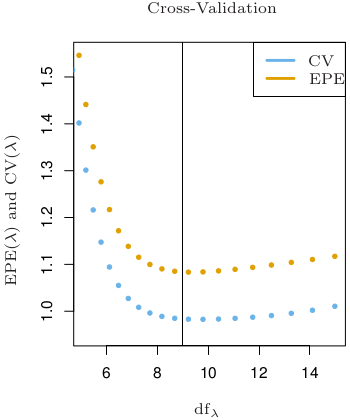
\includegraphics[width=0.55\textwidth]{figure5_9_tl}
}



\subsection{Multidimensional splines}

\frame{\frametitle{Multidimensional splines: }
\framesubtitle{multidimensional splines}
All spline models generalize to \textcolor{uio}{multidimensional} cases.

\vspace{12pt}

Consider $X \in \mathds{R}^2$, then
$$
g(X) = \sum_{j=1}^{M_1} \sum_{k=1}^{M_2} \theta_{jk} g_{jk}(X),
$$
where:
\begin{itemize}
\item $g_{jk}(X)$ is an element of the $M_1 \times M_2$ \textcolor{uio}{tensor product basis}
$$
g_{jk}(X) = h_{1j}(X_1)h_{2k}(X_2), j=1,\dots,M_1, k=1,\dots,M_2;
$$
\item $h_{1j}(X_1)$ is a \textcolor{uio}{set of $M_1$ basis} for the coordinate \textcolor{uio}{$X_1$};
\item $h_{2j}(X_2)$ is a set of \textcolor{uio}{$M_2$ basis} for the coordinate \textcolor{uio}{$X_2$};
\item $\theta = \theta_{jk}$ is the $M_1\times M_2$-dimensional vector of \textcolor{uio}{coefficients}.
\end{itemize}
}


\frame{\frametitle{Multidimensional splines: }
\framesubtitle{multidimensional splines}
\centering
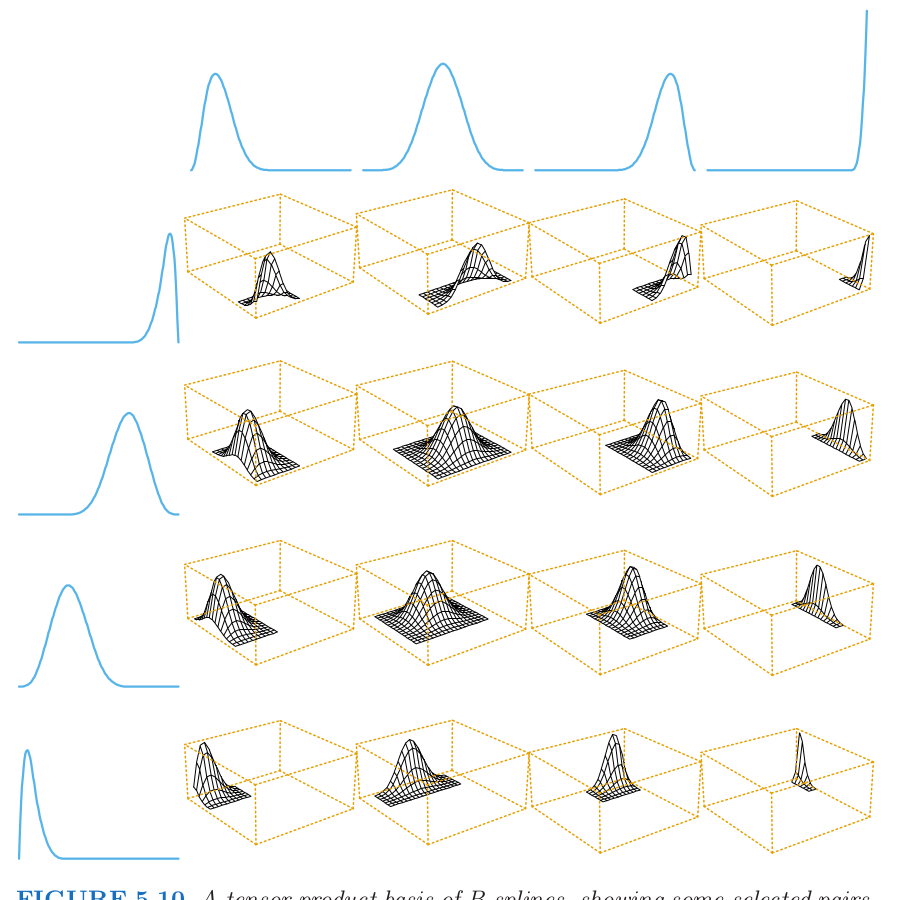
\includegraphics[width=0.72\textwidth]{figure5_10}
}


\frame{\frametitle{Multidimensional splines: }
\framesubtitle{multidimensional smoothing splines}
Smoothing splines can be extended to \textcolor{uio}{more than one} dimension as well, by \textcolor{uio}{generalizing}
$$
\hat{f}(x) = \text{argmin}_{f(x)} \sum_{i = 1}^N \{y_i - f(x_i)\}^2 + \lambda J[f(x)],
$$
where $J[f(x)]$ takes care of the \textcolor{uio}{``smoothness'' in $\mathds{R}^d$}.

\vspace{12pt}

For example, in the case $d=2$,
$$
J[f(x)] = \int_\mathds{R} \int_\mathds{R} \left[\left(\frac{\partial^2 f(x)}{\partial x_1^2}\right)^2 + 2\left(\frac{\partial^2 f(x)}{\partial x_1\partial x_2}\right)^2 + \left(\frac{\partial^2 f(x)}{\partial x_2^2}\right)^2\right]dx_1dx_2.
$$
}


\frame{\frametitle{Multidimensional splines: }
\framesubtitle{multidimensional smoothing splines}
The minimizer $\hat{f}(x)$ (in $\mathds{R}^2$) is known as {\bf thin-plate spline}:
\begin{itemize}
\item for \textcolor{uio}{$\lambda \rightarrow 0$}, $\hat{f}(x) \rightarrow$ \textcolor{uio}{interpolation} function;
\item for \textcolor{uio}{$\lambda \rightarrow \infty$}, $\hat{f}(x) \rightarrow$ \textcolor{uio}{least square} hyperplane;
\item for intermediate values of $\lambda$, linear expansion of basis with their coefficients computed by a form of \textcolor{uio}{generalized ridge}.
\item[]
\end{itemize}
The solution has the form
$$
f(x) = \beta_0 + \beta^Tx + \sum_{j=1}^N \alpha_j h_j(x),
$$
where $h_j(x) = ||x - x_j||²\log ||x-x_j||$ (\textcolor{uio}{radial basis} function).
}


\frame{\frametitle{Multidimensional splines: }
\framesubtitle{multidimensional smoothing splines}
Remarks:
\begin{itemize}
\item the computational \textcolor{uio}{complexity} is \textcolor{uio}{$O(N^3)$};
\item often the thin-plate splines are only computed on a \textcolor{uio}{grid of $K$ knots} distributed on the domain (see figure);
\item the computational complexity \textcolor{uio}{reduces} to \textcolor{uio}{$O(NK^2 + K^3)$};
\end{itemize}
Simplification:
\begin{itemize}
\item by imposing a \textcolor{uio}{specific structure};
\item e.g., \textcolor{uio}{additivity}:
\begin{itemize}
 \item $f(x) = \alpha + f_1(x_1) + \dots + f_d(x_d)$ (\textcolor{uio}{GAM}, see next lecture);
 \item then
 \begin{align*}
  J[f(x)] &= J(f_1(x_1) + \dots + f_d(x_d))\\
  &= \sum_{j=1}^d\int f_j''(t_j) dt_j.
 \end{align*}
 \end{itemize} 
\end{itemize}
}


\frame{\frametitle{Multidimensional splines: }
\framesubtitle{multidimensional smoothing splines}
\centering
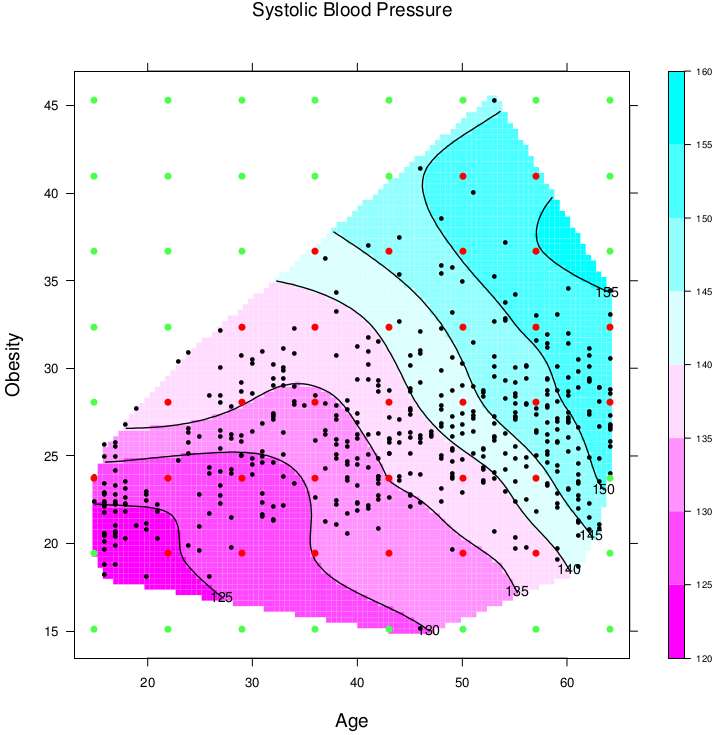
\includegraphics[width=0.7\textwidth]{figure5_12}
}



%%%%%%%%%%%%
%\section*{Bibliography}
%%%%%%%%%%%%
%
%\frame[allowframebreaks]{\frametitle{References}
%\footnotesize
%\bibliographystyle{../../../../support/biometrika}
%\bibliography{../../../../support/biblio}
%}

\end{document}
